\documentclass[10pt,letterpaper]{article}
\usepackage[utf8]{inputenc}
\usepackage[T1]{fontenc}
\usepackage[margin=0.6in]{geometry}
\usepackage{amsmath,amssymb,mathtools,graphicx,booktabs,xcolor,hyperref}
\setlength{\parindent}{0pt}
\setlength{\parskip}{5pt}
\begin{document}

\section*{Block S4 Exercises: DC-Driven Series RLC Circuit Analysis}

  \textbf{Schedule Window:} Sunday, Oct 18, 6:50--7:50 PM (60 min) ~|~
  \textbf{Total Points:} 36 pts ~|~
  \textbf{Mix:} 1 Second-Order ODE Derivation, 1 Spec v2 RLC Step-Response FR, 1 Damping Graph + Cloze



  \textbf{Core Mastery Goals:} (1) Deriving the second-order ODE $LC\frac{d^2 v_C}{dt^2} + RC\frac{dv_C}{dt} + v_C = V_s$, characteristic roots, critical damping resistance $R_{\text{crit}} = 2\sqrt{L/C}$, and ringing frequency $\omega' = \sqrt{\frac{1}{LC} - \frac{R^2}{4L^2}}$; (2) Enforcing dual continuity $v_C(0^+)=v_C(0^-)$ and $i_L(0^+)=i_L(0^-)$ alongside DC steady-state limits ($t \to \infty$: $C =$ open, $L =$ short); (3) Sketching underdamped, critically damped, and overdamped step responses.


\subsection*{01 $\cdot$ Second-Order Series RLC ODE, Characteristic Roots \& Critical Damping Proof \hfill [Ch. 30 $\cdot$ 12 Points $\cdot$ DERIVE]}

A constant DC voltage source $V_s = \mathcal{E}$ is switched at $t = 0$ into a series circuit containing resistance $R$, inductance $L$, and capacitance $C$.

\begin{enumerate}
  \item \textbf{Second-Order Differential Equation in $v_C(t)$ [4 points]:}
    \begin{enumerate}
      \item Write Kirchhoff's loop rule for $t \ge 0$ in terms of the loop current $i(t)$, $\dfrac{di}{dt}$, and the capacitor voltage $v_C(t)$.
      \item Using $q(t) = C v_C(t)$, express $i(t) = \dfrac{dq}{dt}$ and $\dfrac{di}{dt} = \dfrac{d^2 q}{dt^2}$ in terms of derivatives of $v_C(t)$, and substitute them into KVL to prove that $v_C(t)$ satisfies the second-order linear ODE:
      $$LC\frac{d^2 v_C}{dt^2} + RC\frac{dv_C}{dt} + v_C = \mathcal{E} \quad \Longleftrightarrow \quad \frac{d^2 v_C}{dt^2} + \frac{R}{L}\frac{dv_C}{dt} + \frac{1}{LC}v_C = \frac{\mathcal{E}}{LC}.$$
    \end{enumerate}
  
  \item \textbf{Characteristic Equation, Damping Regimes \& $R_{\text{crit}}$ [5 points]:}
    \begin{enumerate}
      \item Substitute the trial homogeneous solution $v_{C,h}(t) = A e^{st}$ into the homogeneous ODE $\frac{d^2 v_{C,h}}{dt^2} + \frac{R}{L}\frac{dv_{C,h}}{dt} + \frac{1}{LC}v_{C,h} = 0$ to obtain the quadratic characteristic equation in $s$, and solve for the roots $s_{1,2}$ in terms of the attenuation constant $\alpha = \dfrac{R}{2L}$ and the undamped natural angular frequency $\omega_0 = \dfrac{1}{\sqrt{LC}}$.
      \item Set the discriminant $\alpha^2 - \omega_0^2 = 0$ to prove that the boundary between oscillatory (underdamped) and non-oscillatory (overdamped) response occurs at the \textbf{critical damping resistance}:
      $$R_{\text{crit}} = 2\sqrt{\frac{L}{C}}.$$
    \end{enumerate}
  
  \item \textbf{Underdamped Ringing Frequency $\omega'$ [3 points]:} When $R < R_{\text{crit}}$, show that the characteristic roots are complex conjugates $s_{1,2} = -\alpha \pm j\omega'$ with damped angular frequency:
  $$\omega' = \sqrt{\omega_0^2 - \alpha^2} = \sqrt{\frac{1}{LC} - \frac{R^2}{4L^2}},$$
  and verify that the general underdamped step response satisfying $v_C(0^+)=0$, $\left.\frac{dv_C}{dt}\right|_{0^+}=0$, and $v_C(\infty)=\mathcal{E}$ is $v_C(t) = \mathcal{E}\left[1 - e^{-\alpha t}\left(\cos(\omega' t) + \frac{\alpha}{\omega'}\sin(\omega' t)\right)\right]$.
\end{enumerate}
\vspace{1.2in}


\newpage



\subsection*{02 $\cdot$ DC Step-Response Continuity ($t=0^+$), Steady State ($t\to\infty$) \& Damping \hfill [Ch. 30 $\cdot$ 14 Points $\cdot$ FR + SPEC V2]}

In the Spec v2 series RLC circuit below, an ideal DC source $V_s = 12.0\text{ V}$ is applied at $t = 0$ to a series combination of $R = 40.0\ \Omega$, $L = 0.800\text{ H}$, and $C = 500\ \mu\text{F}$. Prior to $t = 0$, the capacitor is completely uncharged ($v_C(0^-) = 0\text{ V}$) and the inductor carries zero current ($i(0^-) = 0\text{ A}$).

\begin{center}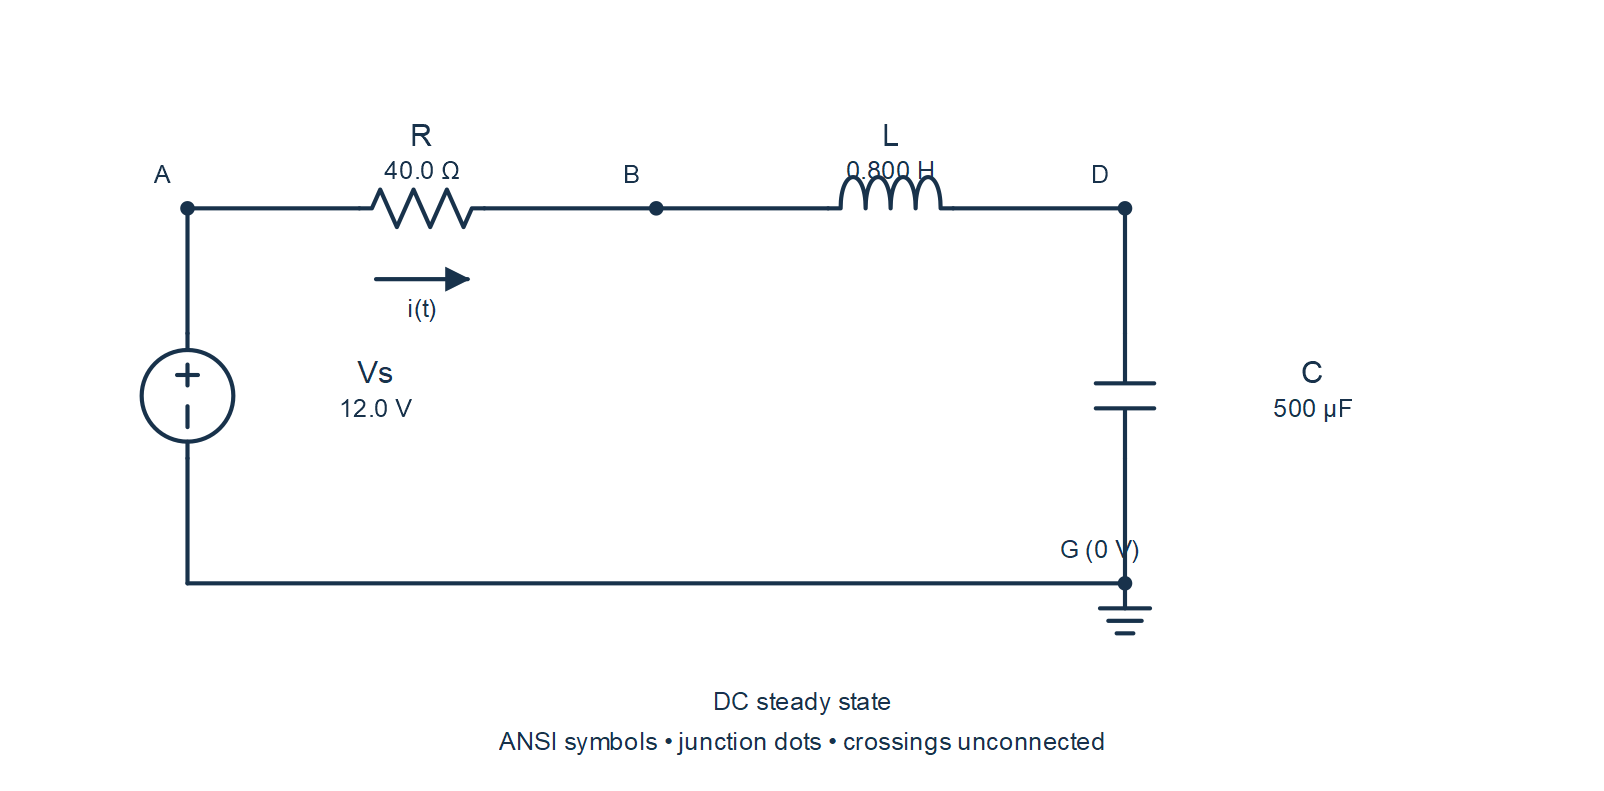
\includegraphics[width=0.82\linewidth]{day1_assets/s4-q2-dc-rlc.png}\end{center}

\begin{enumerate}
  \item \textbf{Initial State Immediately After Switching ($t = 0^+$) [5 points]:}
    \begin{enumerate}
      \item Using the physical continuity rules for an inductor and a capacitor, state $i(0^+)$ (in $\text{A}$) and $v_C(0^+)$ (in $\text{V}$).
      \item Find the initial resistor voltage $v_R(0^+)$ and apply KVL at $t = 0^+$ to determine the initial inductor voltage $v_L(0^+)$ (in $\text{V}$).
      \item Calculate the initial rate of change of current $\left.\dfrac{di}{dt}\right|_{t=0^+}$ (in $\text{A/s}$), the initial rate of change of capacitor voltage $\left.\dfrac{dv_C}{dt}\right|_{t=0^+}$ (in $\text{V/s}$), and the initial second derivative $\left.\dfrac{d^2 v_C}{dt^2}\right|_{t=0^+}$ (in $\text{V/s}^2$).
    \end{enumerate}
  
  \item \textbf{Final DC Steady State ($t \to \infty$) \& Stored Energy [4 points]:}
    \begin{enumerate}
      \item As $t \to \infty$ (after all transients have died out), state the asymptotic circuit model (open circuit vs. short circuit) for $L$ and for $C$, and determine $i(\infty)$, $v_R(\infty)$, $v_L(\infty)$, and $v_C(\infty)$.
      \item Compute the final magnetic energy stored in the inductor $U_L(\infty) = \frac{1}{2}L[i(\infty)]^2$ and the final electric energy stored in the capacitor $U_C(\infty) = \frac{1}{2}C[v_C(\infty)]^2$ (in $\text{mJ}$).
    \end{enumerate}
  
  \item \textbf{Damping Classification \& Peak Overshoot [5 points]:}
    \begin{enumerate}
      \item Calculate the undamped natural frequency $\omega_0 = \frac{1}{\sqrt{LC}}$ (in $\text{rad/s}$), the damping coefficient $\alpha = \frac{R}{2L}$ (in $\text{s}^{-1}$), and the critical damping resistance $R_{\text{crit}} = 2\sqrt{\frac{L}{C}}$ (in $\Omega$).
      \item Classify the circuit at $R = 40.0\ \Omega$ as \emph{underdamped}, \emph{critically damped}, or \emph{overdamped}, compute the damped ringing frequency $\omega' = \sqrt{\omega_0^2 - \alpha^2}$ (in $\text{rad/s}$), and find the time $t_{\text{peak}} = \frac{\pi}{\omega'}$ (in $\text{ms}$) and maximum capacitor voltage $v_{C,\max} = v_C(t_{\text{peak}})$ (in $\text{V}$) at the first overshoot peak.
    \end{enumerate}
  
\end{enumerate}
\vspace{1.2in}


\newpage



\subsection*{03 $\cdot$ Step-Response Damping Curves \& RLC Continuity Cloze \hfill [Ch. 30 $\cdot$ 10 Points $\cdot$ DRAW + CLOZE]}

\subsubsection*{Part A: Draw the Effect --- Underdamped, Critically Damped \& Overdamped Step Responses [6 points --- DRAW]}
For the series RLC circuit of Exercise 02 ($V_s = 12.0\text{ V}, L = 0.800\text{ H}, C = 500\ \mu\text{F}$), sketch on the same coordinate axes below the capacitor voltage $v_C(t)$ (\textbf{dependent variable}, vertical axis, in $\text{V}$) vs. time $t$ (\textbf{independent variable}, horizontal axis, in $\text{ms}$) for $0 \le t \le 150\text{ ms}$ for three different series resistances, identifying the damping regime of each curve:
\begin{enumerate}
  \item \textbf{Curve 1 (Solid): $R_1 = 40.0\ \Omega$} --- state the damping regime, draw the dashed horizontal steady-state asymptote $v_C(\infty)$, and mark the initial slope at $t = 0^+$ along with the coordinates $(t_{\text{peak}}, v_{C,\max})$ of any first peak found in Exercise 02. \textbf{[2.5 pts]}
  \item \textbf{Curve 2 (Dashed): $R_2 = 80.0\ \Omega$} --- state the damping regime and sketch its time response relative to Curve 1 and $v_C(\infty)$. \textbf{[2 pts]}
  \item \textbf{Curve 3 (Dotted): $R_3 = 160\ \Omega$} --- state the damping regime and sketch its time response relative to Curves 1 and 2. \textbf{[1.5 pts]}
\end{enumerate}

\begin{center}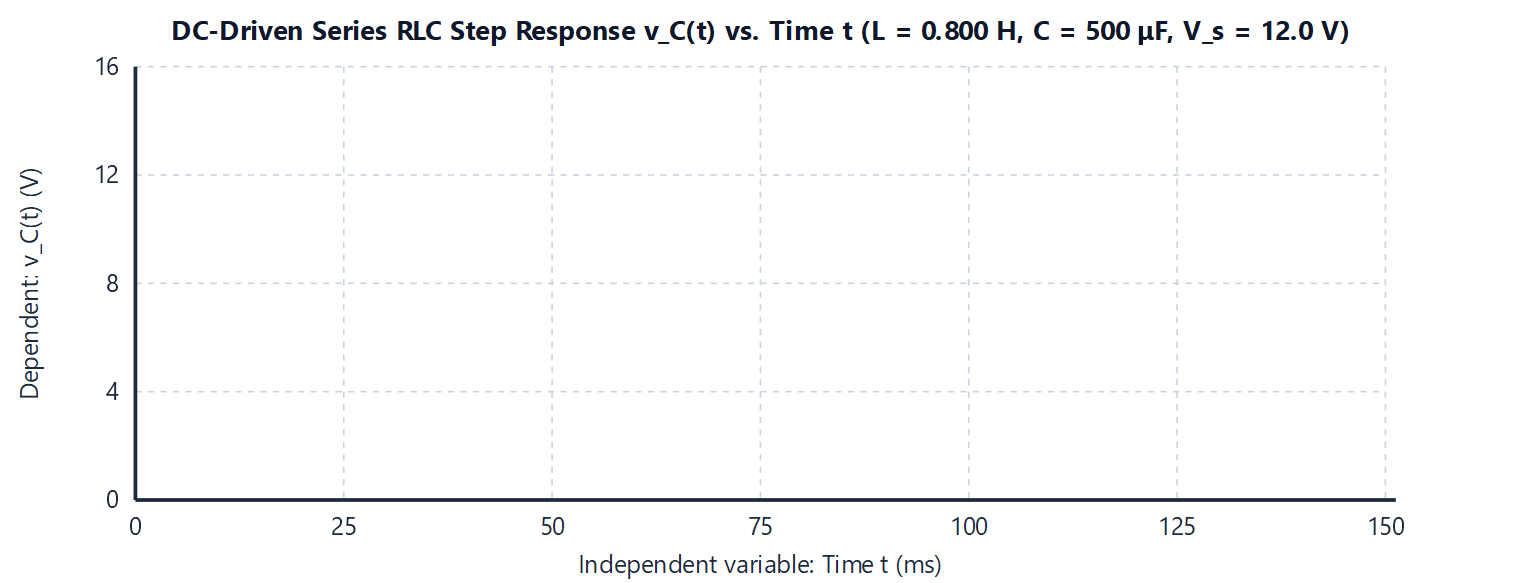
\includegraphics[width=0.82\linewidth]{day1_assets/s4-q3-grid-blank.png}\end{center}

\subsubsection*{Part B: DC-Driven RLC Continuity \& Damping Cloze [4 points --- 0.5 point each]}

  \textbf{WORD BANK:} ~
  \texttt{inductor current $i_L(t)$} $\cdot$
  \texttt{inductor voltage $v_L(t)$} $\cdot$
  \texttt{open circuit} $\cdot$
  \texttt{short circuit} $\cdot$
  \texttt{underdamped} $\cdot$
  \texttt{critically damped} $\cdot$
  \texttt{overdamped} $\cdot$
  \texttt{$2\sqrt{L/C}$} $\cdot$
  \texttt{$1/\sqrt{LC}$} $\cdot$
  \texttt{zero}


\begin{enumerate}
  \item Because magnetic flux linkage $\Phi_B = L i_L$ cannot change instantaneously under a finite voltage ($v_L = L\frac{di_L}{dt}$), the \underline{\hspace{1.8in}} must be continuous across any switching instant, whereas the \underline{\hspace{1.8in}} can jump discontinuously.
  \item At $t = 0^+$ when a DC step voltage is applied to a de-energized inductor ($i_L(0^+)=0$), the inductor momentarily acts like an \underline{\hspace{1.8in}}; as $t \to \infty$ in DC steady state ($\frac{di_L}{dt} = 0$), the ideal inductor acts like a \underline{\hspace{1.8in}}.
  \item Because $i(0^+) = C\left.\frac{dv_C}{dt}\right|_{0^+} = 0$ in a initially de-energized series RLC circuit, the initial slope of the $v_C(t)$ graph at $t = 0^+$ is always \underline{\hspace{1.8in}} for all damping regimes.
  \item The boundary between oscillatory ringing and non-oscillatory decay occurs at $R_{\text{crit}} =$ \underline{\hspace{1.8in}}.
  \item When $0 < R < R_{\text{crit}}$, the circuit is \underline{\hspace{1.8in}} and $v_C(t)$ overshoots and rings around $V_s$; when $R = R_{\text{crit}}$, the circuit is \underline{\hspace{1.8in}} and approaches $V_s$ as rapidly as possible without overshooting.
\end{enumerate}

\end{document}
